\section{Langevin Thermostat}

At first notice that the script ljsim.py was changed in such a way that you can pass more command line parameters via argparse.
The simulation ID is now passes via --ID.\\

The Langevin thermostat simulates a solvent in which causes friction and random forces (through collisions).
It allows to conserve the canonical (N,V,T)-ensemble.\\

\subsection{Implementation}

The implementation of the formulas which were given on the worksheet is done in code block \ref{langevin}.

\listfile{../src/ljsim.py}{src/ljsim.py}{94}{113}{Langevin thermostat}{langevin}

The random force is generated in line 114 with the the function $\ovec{W}_i(t)=\sqrt{12}\sigma\cdot a$ where a is a uniform random number between $-0.5$ and $0.5$ and the standard deviation $\sigma =\sqrt{\frac{2mk_BT\gamma}{\D t}}$.\\

The script allows to take the optional command line argument --gamma which is default $\gamma =0.3$.
Furthermore the main loop is modified in such a way, that it stores the trajectory, the velocities and the temperatures in the *.dat-file, so that you can not only restart the simulation but also get knowledge about the former simulation data.
The new command line parameter --restart allows you to restart a simulation instead of continuing it.

\subsection{Simulation}

Now the simulation can be performed. 
The desired temperature T\_des can be set by --T and is default 1.0.
The result of the simulation is shown as a plot of temperature over time \ref{langevinT}.

\begin{figure}[ht]
	\centering
	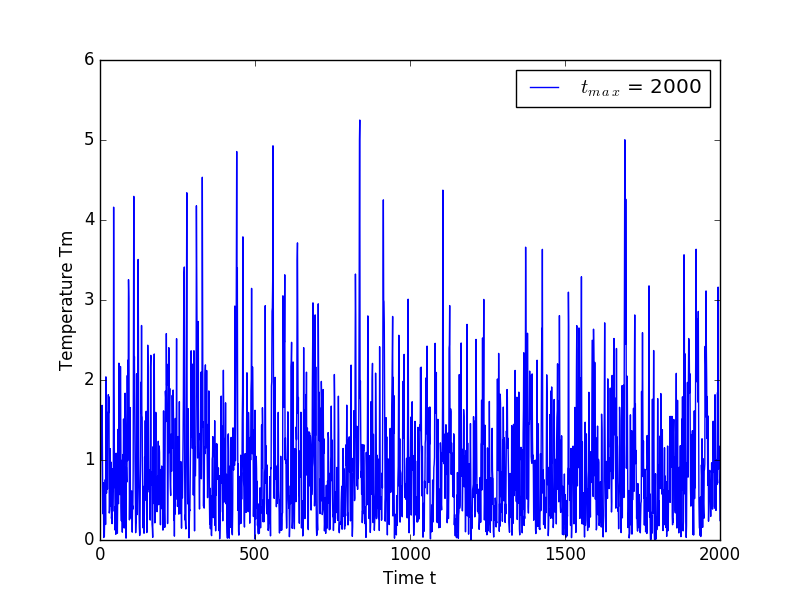
\includegraphics[width=0.7\textwidth]{../dat/langevin_T1d0_gamma0d3_Tm.png}
	\caption{
		Plot of the temperature over time for a desired temperature of $T_\text{des}=1.0$ for a simulation with the Langevin thermostat and $\gamma =0.3$.
	}
	\label{langevinT}
\end{figure}

In order to check weather the Maxwell-Boltzmann distribution for the velocities is fulfilled a histogram of the velocity distribution is drawn in figure \ref{langevinvv}.
Of course the distribution is meant over over time, because we are simulationg only one particle, but the script allows also to get a distribution also over all particles if we set other initial conditions with more than one particle.
For a physical system with Temperature $T$, the deviation is $\sigma =\sqrt{T}$.

\listfile{../src/ljsim.py}{src/ljsim.py}{290}{299}{Calculation of the histogram}{vvhist}

\begin{figure}[ht]
	\centering
	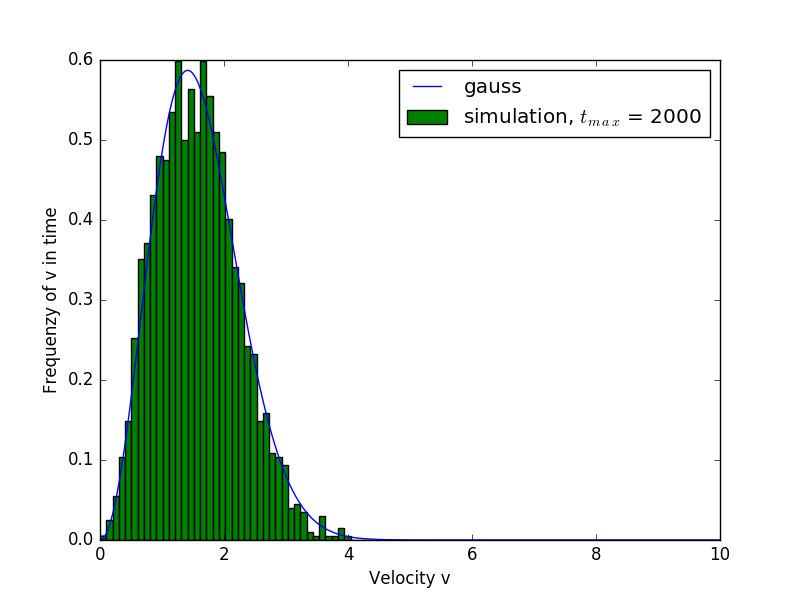
\includegraphics[width=0.7\textwidth]{../dat/langevin_T1d0_gamma0d3_vv.png}
	\caption{
		Histogram for the distribution of the absolute of the velocities in time for a desired temperature of $T_\text{des}=1.0$ for a simulation with the Langevin thermostat and $\gamma =0.3$.
	}
	\label{langevinvv}
\end{figure}

The figures show that the simulated velocity behaves like we physically expect it to behave. 
The temperature is varies around 1.0 with many high peaks in between, but the velocity distribution clearly fits the expected Gaussian.

\FloatBarrier